\chapter{Radiographische Untersuchung von Objekten}
\label{vn:roentgen-1}

In diesem Versuch nehmen Sie Röntgenbilder selbst auf.
%
%------------------------------------------------
\section{Stichworte}
%------------------------------------------------
Röntgenstrahlung, Absorption, Transmission, Fluoreszenz.
%
%------------------------------------------------
\section{Literatur}
%------------------------------------------------
\etodo{Literatur raussuchen}
%
%------------------------------------------------
\section{Anwendungsbeispiele}
%------------------------------------------------
%
Röntgenaufnahmen, Computertomographie, etc
\etodo{Anwendungsbeispiele vernünftig beschreiben}
%
%------------------------------------------------
\section{Theoretischer Hintergrund}
%------------------------------------------------

\subsection{Erzeugung von Röntgenstrahlung}

\subsection{Absorption von Röntgenstrahlung in Materie}

\subsection{Prinzip der Computertomographie}
%------------------------------------------------
\section{Fragen zur Vorbereitung}
%------------------------------------------------

\begin{enumerate} 
	\item Wie wird Röntgenstrahlung erzeugt?
	%
	\item Was ist der Fotoeffekt?
	%
	\item Wie macht ein Fluoreszenzschirm auftreffende Röntgenphotonen sichtbar?
	%
	\item Welche Arten von Materialen lassen sich mittels Transmissionsradiographie unterscheiden?
	%
\end{enumerate} 

%------------------------------------------------
\section{Durchführung} 
%------------------------------------------------

\subsection{Vorbereitung}

\begin{hint}
	Das im Experiment verwendete Röntgengerät ist durch Bleiglas gesichert (Vollschutzgerät). Wird die Fronttür geöffnet, schaltet sich die Röhre automatisch aus. Allerdings sollte man sich beim Betrieb des Geräts nicht unnötig lange in dessen unmittelbarer Nähe ($<$10~cm Abstand) aufhalten.
\end{hint}
%
Montieren Sie den Fluoreszenzschirm und den Objekthalter auf der optischen Bank im Inneren des Röntgengerätes. \\
Dabei ist der Fluoreszenzschirm so weit rechts in der Kammer wie möglich aufzubauen. Zur Positionierung des Objekthalters bedenken Sie, dass es durch den Öffnungswinkel des Strahls zu einer Vergrößerung der Abbildung des Objektes kommt. Das bedeutet, dass große Objekte nahe am Schirm sein sollten, damit die gesamte Abbildung auf dem Schirm liegt, während kleine Objekte weiter vom Schirm entfernt sein können. Zusammen mit der Vergrößerung des Objektes wird die Abbildung bei größerem Abstand allerdings auch unschärfer, was Sie  bei der Positionierung ebenfalls bedenken sollten.

\begin{jason}
	Betreiben Sie das Gerät für die ersten zehn Minuten des Versuchs bei einer maximalen Anodenspannung von 25~kV. Dies trägt zur Lebensdauer der Röntgenröhre bei.
\end{jason}

\begin{figure}[h!]
	\begin{center}
		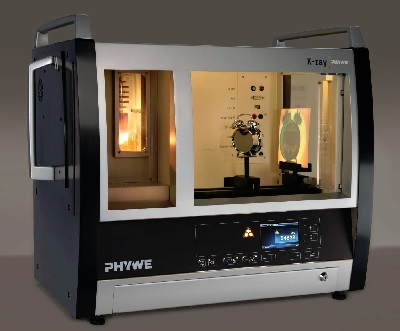
\includegraphics[width=0.90\textwidth]{figures/roentgen-ueberblick.jpg}
	\end{center}
\end{figure}

\subsubsection{Aufnahme von Fotos}

Die Betreuer händigen Ihnen vor Beginn des Versuchs eine der zugehörigen Digitalkameras aus. 
\begin{itemize}
	\item Montieren Sie diese auf der Kamerahalterung außerhalb der Box so, dass der Fluoreszenzschirm den Aufnahmebereich komplett ausfüllt.
	\item Schalten Sie die Kamera in Nachtmodus und deaktivieren Sie den Blitz.
	\item Verdunkeln Sie den Raum.
	\item Es wird empfohlen, die Aufnahme mittels der beiliegenden Fernbedienung auszulösen, damit die Bilder nicht verwackeln, wenn Sie auf den Auslöserknopf der Kamera drücken.
\end{itemize}

\subsection{Durchführung}

\begin{enumerate}
	\item 
	%
\end{enumerate}


%------------------------------------------------
\section{Auswertung} 
%------------------------------------------------
\etodo{Musterauswertung}

\begin{enumerate}
	\item
\end{enumerate}